\documentclass[12pt]{article}
\usepackage[top=1in,bottom=1in,left=1in,right=1in]{geometry}
\usepackage{alltt}
\usepackage{array}
\usepackage{graphicx}
\usepackage{tabularx}
\usepackage{verbatim}
\usepackage{setspace}
\usepackage{listings}
\usepackage{amssymb,amsmath, amsthm}
\usepackage{qtree}
\usepackage{hyperref}
\usepackage{oz}
\usepackage[cc]{titlepic}
\usepackage{fancyvrb}
\usepackage{epstopdf}

\title{SOEN 331 (Section S): Introduction to Formal Methods\\for Software Engineering\\
\ \\
Assignment 3 on Temporal Logic}
\author{\textbf{Gordon Pham-Nguyen}\\
		\texttt{40018402}
\ \\
\textbf{Jeffrey Li}\\
		\texttt{id}
\ \\
\textbf{Tabesh Haidary}\\
		\texttt{id}
\ \\
\textbf{Ian Phillips}\\
		\texttt{id}
\ \\
}
\date{\today}

\begin{spacing}{1.5}
\begin{document}
\maketitle

\newpage

\section*{Problem 1 (20 pts):  Analyzing program behavior}

\begin{enumerate}

\item (10 pts) Visualize all models of behavior.

\begin{figure}[h!]
  \centering
  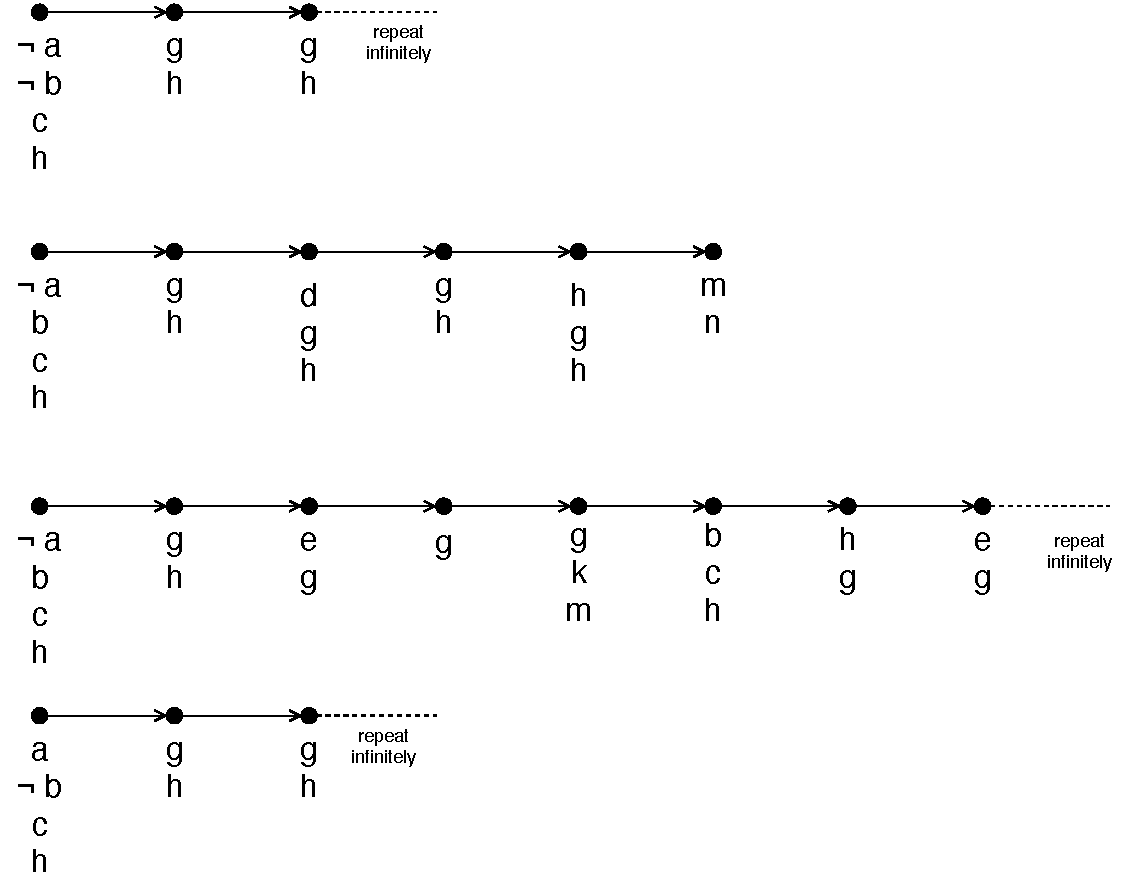
\includegraphics[width=0.9\textwidth]{figures/1_1.pdf}
 \end{figure}

\item (3 pts) Specify conditions (model of behavior), if any exist, under which the program can terminate\dots

The 2nd model is the only model that terminates.

\item (7 pts) For the expressions below, indicate (true/false) whether there exists a
model where the expression holds. When true, cross reference your particular model:

\begin{table}
\centering
\begin{tabular}{|l|l|}
\hline
\textbf{PROPERTY}							& \textbf{TRUE/FALSE}\\
\hline

$(a \wedge c) \rightarrow \Diamond \Box (g \wedge h)$	 &TRUE \#4\\

&\\

\hline

&\\

$h ~\mathcal{U}~ m$									 &TRUE \#2\\

&\\

\hline

&\\

$h ~\mathcal{U}~ (k \wedge g)$						 &FALSE\\

&\\

\hline

&\\

$(b \wedge c) \rightarrow \Box \Diamond (b \wedge c)$  &TRUE \#3\\

&\\

\hline

&\\

$(k \wedge \bigcirc (k \wedge g)) \rightarrow \bigcirc m$  &FALSE\\

&\\

\hline

&\\

$ h ~\mathcal{S}~ c$								 &TRUE \#1 \#2 \#4\\

&\\

\hline

&\\

$ ((g \wedge h) \wedge \bigcirc d) \rightarrow \bigcirc^{2} (g \wedge h)$  &TRUE \#2\\

&\\

\hline

&\\

$e ~\mathcal{R}~ h$									 &FALSE\\

&\\

\hline

&\\

The program has the following stability property: &FALSE\\
$\Diamond \Box (b \wedge \ c \wedge h)$		 &\\

&\\

\hline

&\\

The program has the following response property: &TRUE \#3\\
$\Box \Diamond (b \wedge \ c \wedge h)$		 &\\

&\\

\hline

&\\

$( g \wedge h)$ is an invariant property of the program.  &FALSE\\

&\\

\hline

&\\

There is a guarantee that $(g \wedge k \wedge h)$	 &TRUE \#2\\

&\\

\hline

&\\

The program has the following response property: &\\
$(b \wedge c \wedge h) \rightarrow \Diamond (b \wedge c \wedge h)$.   &TRUE \#3\\

&\\

\hline

\end{tabular}
\end{table}

\newpage

\begin{table}
	\centering
	\begin{tabular}{|l|l|}
	\hline
	\textbf{PROPERTY}							& \textbf{TRUE/FALSE}\\
	\hline
	&\\

The program has the following precedence property: &\\
$(b \wedge c \wedge h) \rightarrow ( (g \wedge h) ~\mathcal{U}~ b \wedge c \wedge h))$
			 &FALSE\\
&\\

\hline
\end{tabular}
\end{table}

\end{enumerate}

\newpage

\section*{Problem 2 (20 pts) :  Visualizing temporal expressions}

\begin{enumerate}

	\item $\Box (\phi \rightarrow \bigcirc^{2} \psi)$

  \begin{figure}[h!]
   \centering
   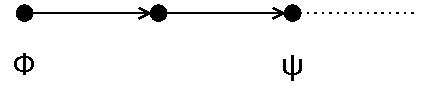
\includegraphics[width=0.9\textwidth]{figures/2_1.pdf}
  \end{figure}

	\item $\Box \phi \rightarrow \bigcirc \psi$

  \begin{figure}[h!]
   \centering
   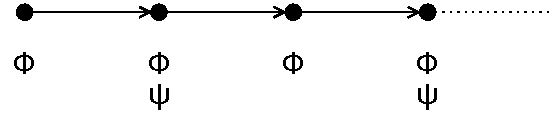
\includegraphics[width=0.9\textwidth]{figures/2_2.pdf}
  \end{figure}

	\item $\phi \rightarrow \bigcirc \Diamond \Box \psi$

  \begin{figure}[h!]
    \centering
    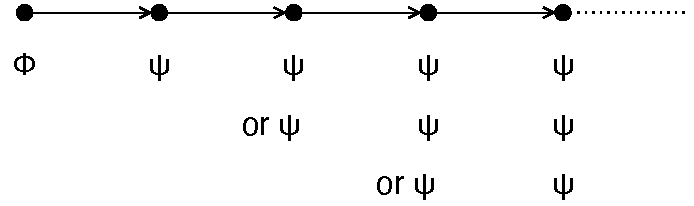
\includegraphics[width=0.9\textwidth]{figures/2_3.pdf}
   \end{figure}

  \newpage

	\item $(\phi \wedge \bigcirc \psi) \rightarrow \bigcirc^{2} \Diamond \Box \omega$

  \begin{figure}[h!]
    \centering
    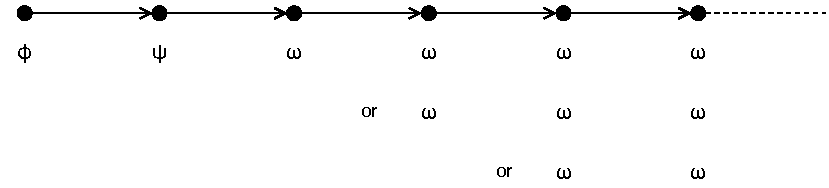
\includegraphics[width=0.9\textwidth]{figures/2_4.pdf}
   \end{figure}

	\item $\Box ((\phi \wedge \bigcirc \psi) \rightarrow \bigcirc^{2} \Diamond \Box \omega)$

	\item $(\phi \wedge \bigcirc \psi) \rightarrow \tau ~\mathcal{R}~ \upsilon$

	\item $(\phi \wedge \bigcirc \psi) \rightarrow \bigcirc (\tau ~\mathcal{R}~ \upsilon)$

	\item $(\phi \wedge \bigcirc \psi) \rightarrow \bigcirc (x ~\mathcal{U}~ \tau)$

	\item $(\phi \wedge \Box \psi) \rightarrow \bigcirc^{2} \Diamond \omega$

	\item $(\phi \wedge \bigcirc^{2} \psi) \rightarrow \bigcirc \Box \omega$

\end{enumerate}

\end{spacing}
\end{document}
